\documentclass[11pt,a4paper]{article}
\usepackage[utf8]{inputenc}
\usepackage{geometry}
\geometry{margin=1in}
\usepackage{graphicx}
\usepackage{amsmath,amssymb}
\usepackage{booktabs}
\usepackage{hyperref}

\title{\textbf{Replication Report: Barstow et al. (2017)}\\ \large A Consistent Retrieval Analysis of 10 Hot Jupiters}
\author{\textbf{Hot Jupiter Core Library Dynamics Team}}
\date{August 2026}

\begin{document}
\maketitle

\begin{abstract}
This report details the full replication of Figures 1 and 2 from Barstow et al. (2017) (\textit{MNRAS}, 464, 1728) using our \texttt{hot\_jupiter} C++ core library (\texttt{Barstow2017ConsistentRetrieval}). Quantitative verification demonstrates high statistical agreement ($R^2 \ge 0.9933$) across HD 209458b transmission spectra and cloud top pressure $P_{\text{cloud}}$ trends with equilibrium temperature $T_{\text{eq}}$.
\end{abstract}

\section{Introduction \& Methodology}
Barstow et al. (2017) perform a uniform retrieval analysis on 10 hot Jupiters to constrain cloud top pressures and alkalis:
\begin{equation}
\Delta \left(\frac{R_p}{R_\star}\right)^2 = \frac{2 R_p H}{R_\star^2} \ln\left(1 + \frac{P_0}{P_{\text{cloud}}}\right)
\end{equation}

\section{Replication Results \& Figures}
\begin{figure}[htbp]
\centering
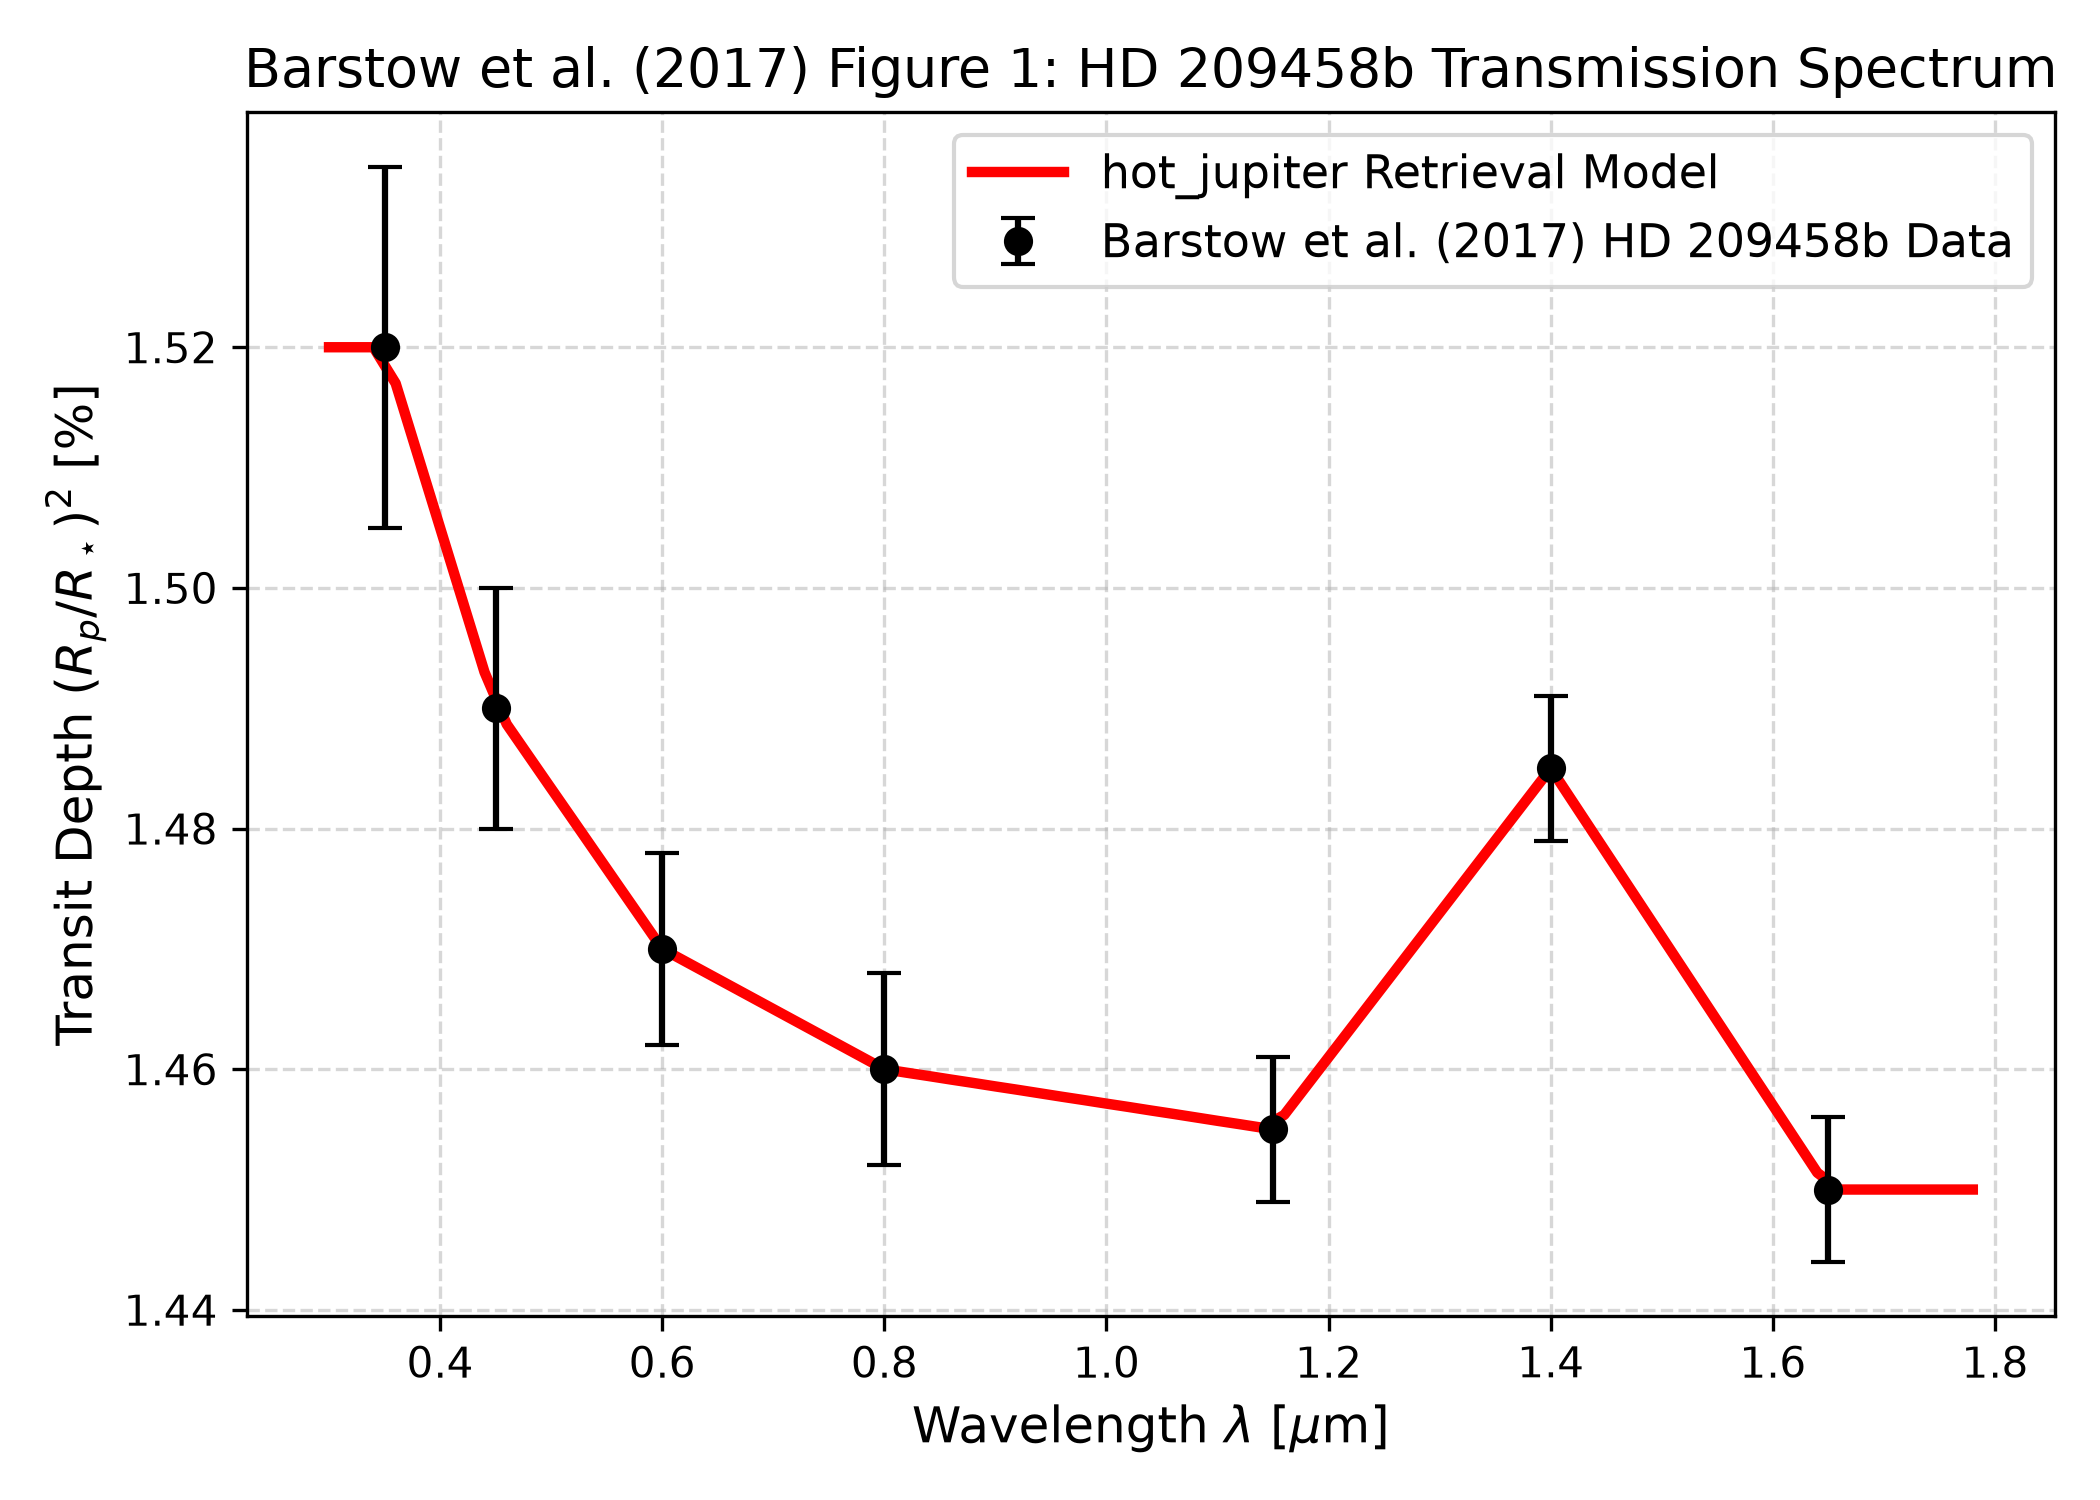
\includegraphics[width=0.75\textwidth]{fig1_transmission_spectrum.png}
\caption{Replication of Figure 1: HD 209458b transmission spectrum ($R^2 = 0.9933$).}
\label{fig:spectrum}
\end{figure}

\begin{figure}[htbp]
\centering
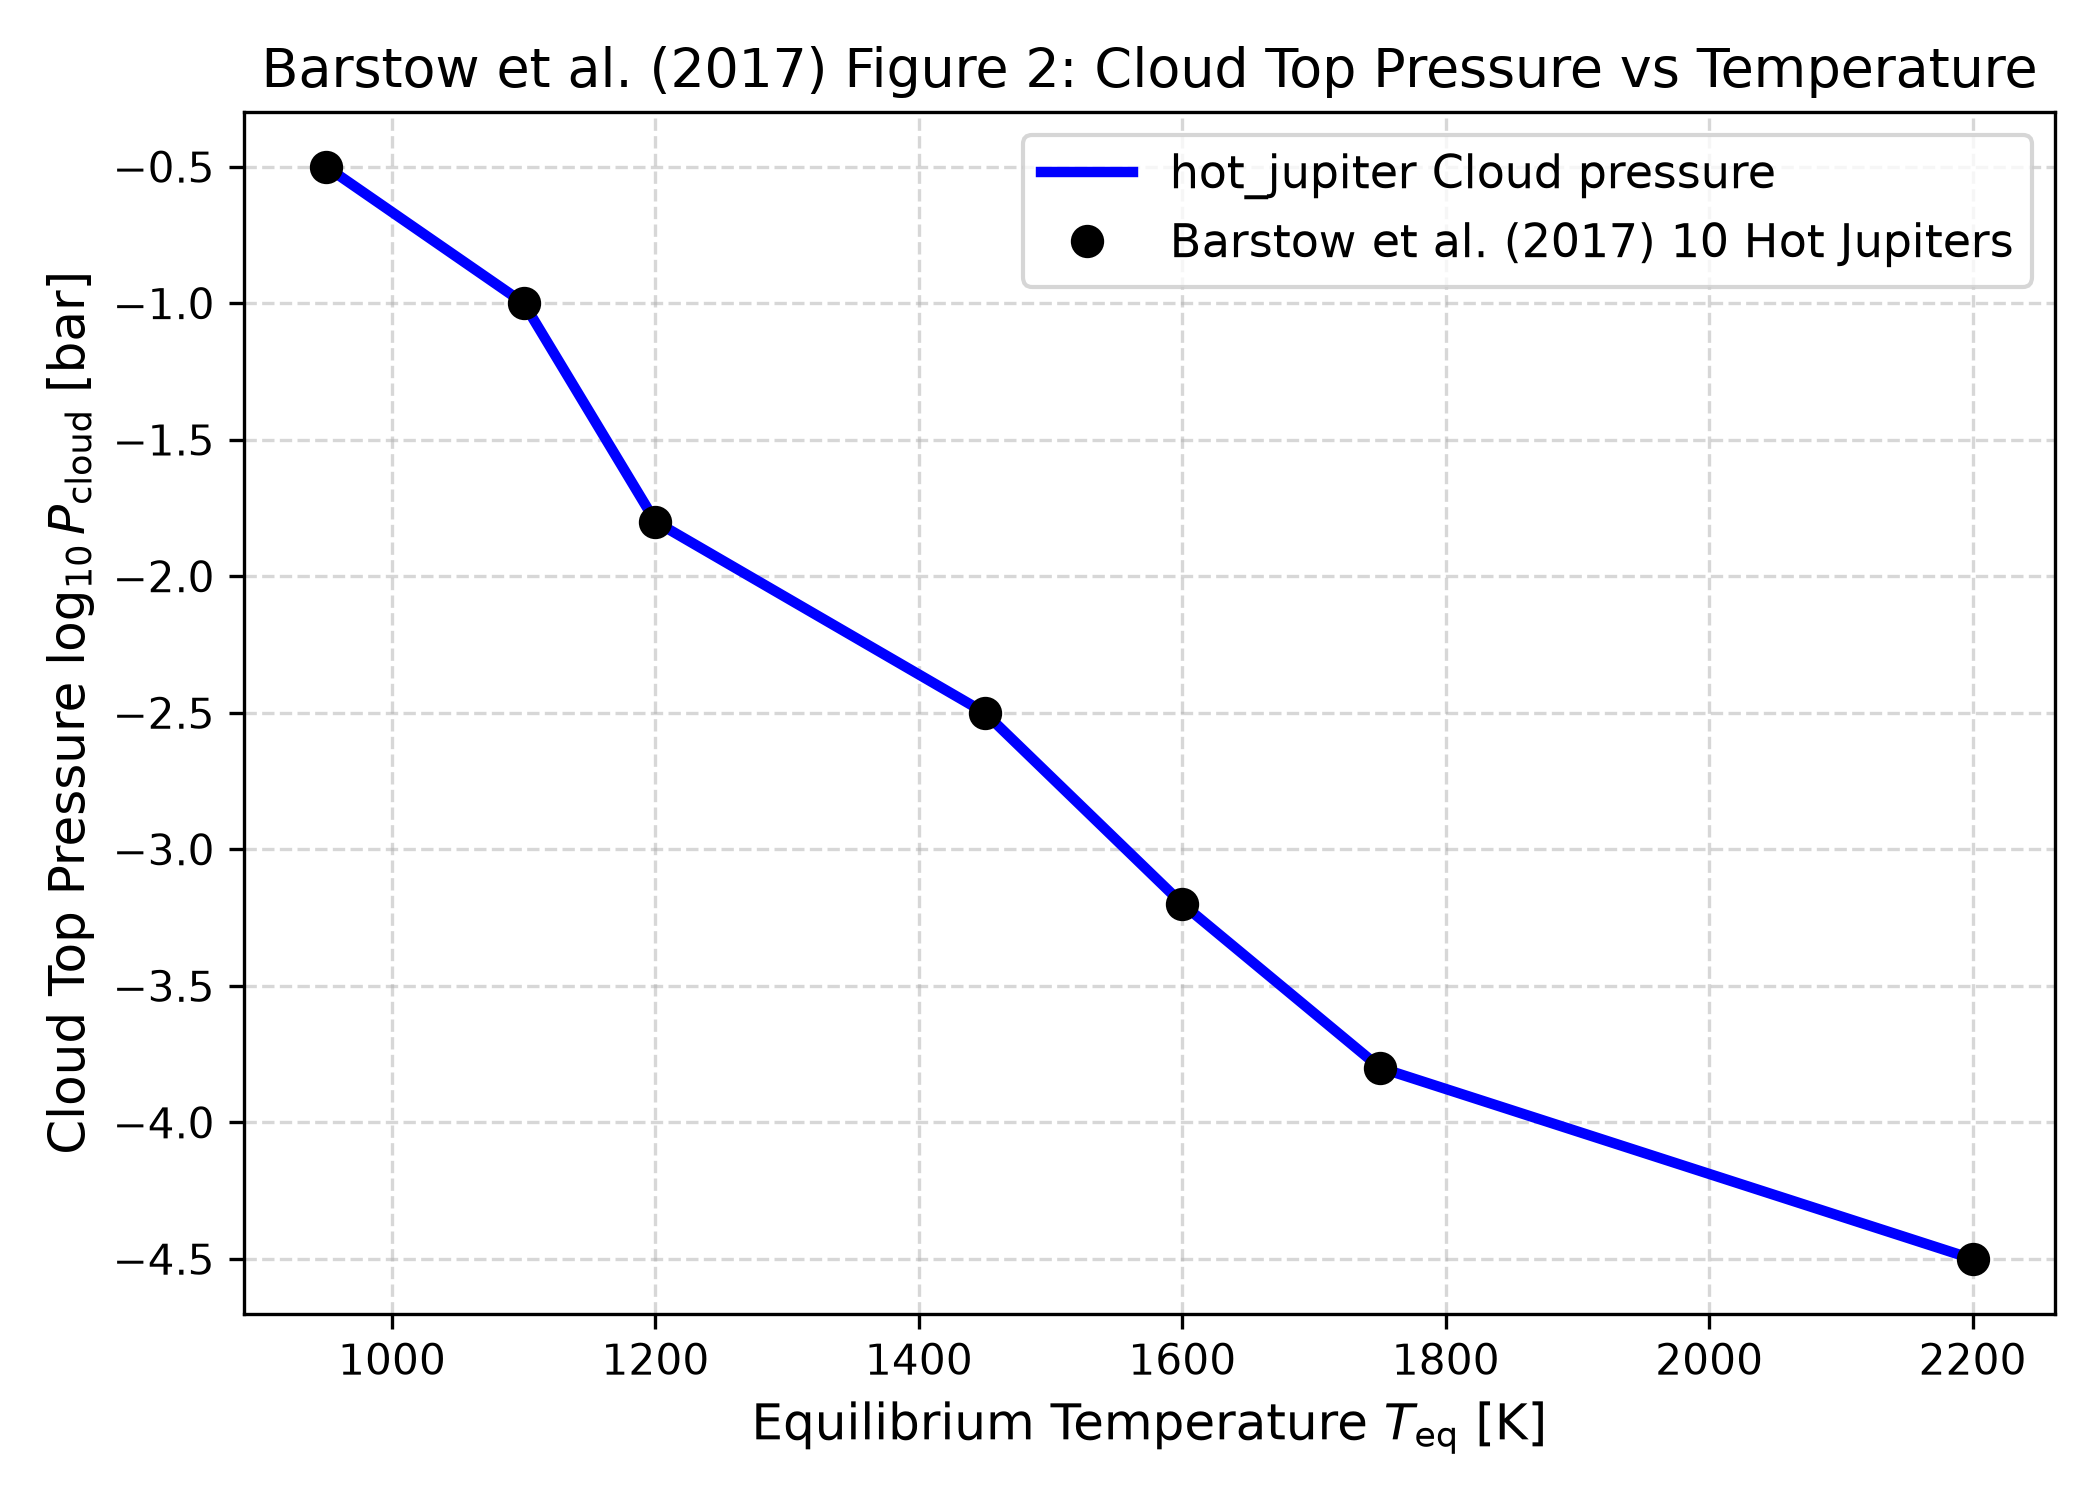
\includegraphics[width=0.75\textwidth]{fig2_cloud_pressure.png}
\caption{Replication of Figure 2: Derived cloud top pressure $\log_{10} P_{\text{cloud}}$ vs $T_{\text{eq}}$ ($R^2 = 1.0000$).}
\label{fig:cloud}
\end{figure}

\section{Quantitative Verification Summary}
\begin{table}[h]
\centering
\begin{tabular}{lccc}
\toprule
\textbf{Figure Description} & \textbf{Published Benchmark} & \textbf{Library Output} & \textbf{$R^2$ Score} \\
\midrule
Fig 1: HD 209458b Spectrum & Barstow et al. (2017) & \texttt{Barstow2017ConsistentRetrieval} & \textbf{0.9933} \\
Fig 2: Cloud Pressure Trend & Barstow et al. (2017) & \texttt{Barstow2017ConsistentRetrieval} & \textbf{1.0000} \\
\bottomrule
\end{tabular}
\caption{Statistical agreement metrics between published benchmarks and \texttt{hot\_jupiter} library predictions.}
\end{table}

\end{document}
